\newpage



\section{MCTS Planning}
\label{sec:mcts_app}
We adapt MCTS to search for the optimal reasoning path (Algorithm~\ref{alg:mcts}). Compared with traditional applications of MCTS, we are faced with a large reasoning space, and the heavy computational cost of LLMs. Thus, we made several modifications to the classic MCTS in our implementation: (1) For open domain problems, e.g., math problems, it's impossible to enumerate all actions (subquestions), so we reduce the action space by sampling a fixed number of potential actions from LLMs, conditioned on a prompt of the current state and in-context demonstration. (2) In the selection phase, if there are actions that haven't been visited before, we estimate the Q value with lightweight local rewards, e.g., self-evaluation reward, and then select the action with UCT. This provides prior knowledge for the exploration, which is crucial given the limited iteration budgets.


\begin{algorithm*}[t]
\centering
\caption{RAP-MCTS}\label{alg:mcts}
\begin{minipage}{0.9\linewidth} 
\small
\begin{algorithmic}[1]
    \Require Initial state $s_0$, state transition probability function $p_\theta$, reward function $r_\theta$, action generator $p_\phi$, number of generated actions $d$, depth limit $L$, number of roll-outs $N$, and exploration weight $w$
    % \Statex
    \State Initialize memory of actions $A : \mathcal S \mapsto \mathcal A$, children $c : \mathcal S \times \mathcal A \mapsto \mathcal S$ 
    and rewards $r : \mathcal S \times \mathcal A \mapsto \mathbb R$ \State Initialize the state-action value function $Q : \mathcal S \times \mathcal A \mapsto \mathbb R$ and visit counter $N : \mathcal S \mapsto \mathbb N$
    \For {$n \gets 0, \dots, N - 1$}
        \State $t \gets 0$
        \While {$N(s_t) > 0$} \Comment{Selection}
            \State $N(s_t) \gets N(s_t) + 1$
            \State $a_t \gets \arg\max_{a \in A(s_t)} \left[ Q(s_t, a) + w \sqrt{\frac{\ln N(s_t)}{N(c(s_t, a))}} \right]$
            \State $r_t = r(s_t, a_t)$, $s_{t+1} \gets c(s_t, a_t)$
            \State $t \gets t + 1$
        \EndWhile
        \While {$s_t$ is not a terminal state $\wedge$ $t \leq L$}
            \For {$i \gets 1, \dots, d$} \Comment{Expansion}
                \State Sample $a_t^{(i)} \sim p_\phi(a \mid s_t)$, $s_{t+1}^{(i)} \sim p_\theta(s_t, a_t^{(i)})$, and $r_t^{(i)} \sim r_\theta(s_t, a_t^{(i)})$
                \State Update $A(s_t) \gets \{a_t^{(i)}\}_{i=1}^d$, $c(s_t, a_t^{(i)}) \gets s_{t+1}^{(i)}$, and $r(s_t, a_t) \gets r_t^{(i)}$
            \EndFor
            \State $a_{t+1} \gets \arg \max_{a \in A(s_t)} r(s_t, a_t)$ \Comment{Simulation}
            \State $r_t \gets r(s_t, a_t)$, $s_{t+1} \gets c(s_t, a_t)$
            \State $t \gets t + 1$
        \EndWhile
        \For {$t' \gets t, \dots, 0$} \Comment{Back propagation}
            \State Update $Q(s_{t'}, a_{t'})$ with $\{r_{t'}, r_{t'+1}, \dots, r_t\}$
        \EndFor
    \EndFor
\end{algorithmic}
\end{minipage}
\end{algorithm*}

\section{Experiment Settings}
\label{sec:details}
\subsection{Language Model Decoding}
We use random sampling with a temperature of 0.8. The generation is cut off at the maximum length of 2048 or a newline token.

\subsection{Computing Resources}
All of our experiments run on 4 $\times$ NVIDIA A5000 GPUs with 24GB memory.

\section{Prompt}
\label{sec:prompt}
\subsection{Plan Generation}
\label{sec:bw_prompt}
We show the prompt to calculate the action likelihood for RAP below. The same prompt is also applied in CoT baseline. \texttt{<init\_state>} and \texttt{<goals>} would be instantiated by the problem to solve.
\begin{lstlisting}[breaklines=true,breakatwhitespace=true]
I am playing with a set of blocks where I need to arrange the blocks into stacks. Here are the actions I can do

Pick up a block
Unstack a block from on top of another block
Put down a block
Stack a block on top of another block

I have the following restrictions on my actions:
I can only pick up or unstack one block at a time.
I can only pick up or unstack a block if my hand is empty.
I can only pick up a block if the block is on the table and the block is clear. A block is clear if the block has no other blocks on top of it and if the block is not picked up.
I can only unstack a block from on top of another block if the block I am unstacking was really on top of the other block.
I can only unstack a block from on top of another block if the block I am unstacking is clear.
Once I pick up or unstack a block, I am holding the block.
I can only put down a block that I am holding.
I can only stack a block on top of another block if I am holding the block being stacked.
I can only stack a block on top of another block if the block onto which I am stacking the block is clear.
Once I put down or stack a block, my hand becomes empty.

[STATEMENT]
As initial conditions I have that, the red block is clear, the yellow block is clear, the hand is empty, the red block is on top of the blue block, the yellow block is on top of the orange block, the blue block is on the table and the orange block is on the table.
My goal is to have that the orange block is on top of the red block.

My plan is as follows:

[PLAN]
unstack the yellow block from on top of the orange block
put down the yellow block
pick up the orange block
stack the orange block on top of the red block
[PLAN END]

[STATEMENT]
As initial conditions I have that, the orange block is clear, the yellow block is clear, the hand is empty, the blue block is on top of the red block, the orange block is on top of the blue block, the red block is on the table and the yellow block is on the table.
My goal is to have that the blue block is on top of the red block and the yellow block is on top of the orange block.

My plan is as follows:

[PLAN]
pick up the yellow block
stack the yellow block on top of the orange block
[PLAN END]

[STATEMENT]
As initial conditions I have that, the red block is clear, the blue block is clear, the orange block is clear, the hand is empty, the blue block is on top of the yellow block, the red block is on the table, the orange block is on the table and the yellow block is on the table.
My goal is to have that the blue block is on top of the orange block and the yellow block is on top of the red block.

My plan is as follows:

[PLAN]
unstack the blue block from on top of the yellow block
stack the blue block on top of the orange block
pick up the yellow block
stack the yellow block on top of the red block
[PLAN END]

[STATEMENT]
As initial conditions I have that, the red block is clear, the blue block is clear, the yellow block is clear, the hand is empty, the yellow block is on top of the orange block, the red block is on the table, the blue block is on the table and the orange block is on the table.
My goal is to have that the orange block is on top of the blue block and the yellow block is on top of the red block.

My plan is as follows:

[PLAN]
unstack the yellow block from on top of the orange block
stack the yellow block on top of the red block
pick up the orange block
stack the orange block on top of the blue block
[PLAN END]

[STATEMENT]
As initial conditions I have that, <initial_state>
My goal is to have that <goals>.

My plan is as follows:

[PLAN]
\end{lstlisting}

For the next state prediction with the world model, we apply the prompts conditioned on the last action. Here we show the prompt to update the state after a ``\texttt{pick up}'' action as an example. Again, \texttt{<state>} and \texttt{<action>} would be instantiated with the current state and action.

\begin{lstlisting}[breaklines=true,breakatwhitespace=true]
I am playing with a set of blocks where I need to arrange the blocks into stacks. Here are the actions I can do 

Pick up a block 
Unstack a block from on top of another block 
Put down a block 
Stack a block on top of another block 

I have the following restrictions on my actions:
I can only pick up or unstack one block at a time. 
I can only pick up or unstack a block if my hand is empty. 
I can only pick up a block if the block is on the table and the block is clear. A block is clear if the block has no other blocks on top of it and if the block is not picked up. 
I can only unstack a block from on top of another block if the block I am unstacking was really on top of the other block. 
I can only unstack a block from on top of another block if the block I am unstacking is clear. Once I pick up or unstack a block, I am holding the block. 
I can only put down a block that I am holding. 
I can only stack a block on top of another block if I am holding the block being stacked. 
I can only stack a block on top of another block if the block onto which I am stacking the block is clear. Once I put down or stack a block, my hand becomes empty.

After being given an initial state and an action, give the new state after performing the action.

[SCENARIO 1]
[STATE 0] I have that, the white block is clear, the cyan block is clear, the brown block is clear, the hand is empty, the white block is on top of the purple block, the purple block is on the table, the cyan block is on the table and the brown block is on the table.
[ACTION] Pick up the brown block.
[CHANGE] The hand was empty and is now holding the brown block, the brown block was on the table and is now in the hand, and the brown block is no longer clear.
[STATE 1] I have that, the white block is clear, the cyan block is clear, the brown block is in the hand, the hand is holding the brown block, the white block is on top of the purple block, the purple block is on the table and the cyan block is on the table.

[SCENARIO 2]
[STATE 0] I have that, the purple block is clear, the cyan block is clear, the white block is clear, the hand is empty, the white block is on top of the brown block, the purple block is on the table, the cyan block is on the table and the brown block is on the table.
[ACTION] Pick up the cyan block.
[CHANGE] The hand was empty and is now holding the cyan block, the cyan block was on the table and is now in the hand, and the cyan block is no longer clear.
[STATE 1] I have that, the cyan block is in the hand, the white block is clear, the purple block is clear, the hand is holding the cyan block, the white block is on top of the brown block, the purple block is on the table and the brown block is on the table.

[SCENARIO 3]
[STATE 0] <state>
[ACTION] <action>
[CHANGE]
\end{lstlisting}

\subsection{Math Reasoning}
We show the prompt of RAP for math reasoning as below. The prompt is used for both action proposal and next state prediction. After instantiate \texttt{<question>}, we append a prefix \texttt{Question 5.1} to the prompt, so that we can sample the first action with the LLM. The future actions are sampled similarly, except that all previous sub-questions and sub-answers need to be appended to the prompt, following the formats of in-context demonstration. The next state prediction, i.e., answering the sub-question, works in the same way.

\begin{lstlisting}[breaklines=true,breakatwhitespace=true]
Given a question, please decompose it into sub-questions. For each sub-question, please answer it in a complete sentence, ending with "The answer is". When the original question is answerable, please start the subquestion with "Now we can answer the question: ".

Question 1: Four years ago, Kody was only half as old as Mohamed. If Mohamed is currently twice as 30 years old, how old is Kody?
Question 1.1: How old is Mohamed?
Answer 1.1: He is currently 30 * 2 = 60 years old. The answer is 60.
Question 1.2: How old was Mohamed four years ago?
Answer 1.2: Four years ago, he must have been 60 - 4 = 56 years old. The answer is 56.
Question 1.3: How old was Kody four years ago?
Answer 1.3: Kody was half as old as Mohamed four years ago. Thus, Kody was 56 / 2 = 28 years old. The answer is 28.
Question 1.4: Now we can answer the question: How old is Kody?
Answer 1.4: She is currently 28 + 4 = 32 years old. The answer is 32.

Question 2: On a moonless night, three fireflies danced in the evening breeze. They were joined by four less than a dozen more fireflies before two of the fireflies flew away. How many fireflies remained?
Question 2.1: How many fireflies joined?
Answer 2.1: The fireflies were joined by four less than a dozen more fireflies, which are 12 - 4 = 8 fireflies. The answer is 8.
Question 2.2: Now we can answer the question: How many fireflies remained?
Answer 2.2: Three fireflies were dancing originally. They were joined by 8 fireflies before two of them flew away. So there were 3 + 8 - 2 = 9 remaining. The answer is 9.

Question 3: Ali has four $10 bills and six $20 bills that he saved after working for Mr. James on his farm. Ali gives her sister half of the total money he has and uses 3/5 of the remaining amount of money to buy dinner. Calculate the amount of money he has after buying the dinner.
Question 3.1: How much money does Ali have in total?
Answer 3.1: Ali has four $10 bills and six $20 bills. So he has 4 * 10 + 6 * 20 = 160 dollars. The answer is 160.
Question 3.2: How much money does Ali give to his sister?
Answer 3.2: Ali gives half of the total money he has to his sister. So he gives 160 / 2 = 80 dollars to his sister. The answer is 80.
Question 3.3: How much money does Ali have after giving his sister the money?
Answer 3.3: After giving his sister the money, Ali has 160 - 80 = 80 dollars left. The answer is 80.
Question 3.4: How much money does Ali use to buy dinner?
Answer 3.4: Ali uses 3/5 of the remaining amount of money to buy dinner. So he uses 80 * 3/5 = 48 dollars to buy dinner. The answer is 48.
Question 3.5: Now we can answer the question: How much money does Ali have after buying the dinner?
Answer 3.5: After buying the dinner, Ali has 80 - 48 = 32 dollars left. The answer is 32.

Question 4: A car is driving through a tunnel with many turns. After a while, the car must travel through a ring that requires a total of 4 right-hand turns. After the 1st turn, it travels 5 meters. After the 2nd turn, it travels 8 meters. After the 3rd turn, it travels a little further and at the 4th turn, it immediately exits the tunnel. If the car has driven a total of 23 meters around the ring, how far did it have to travel after the 3rd turn?
Question 4.1: How far did the car travel except for the 3rd turn?
Answer 4.1: It travels 5 meters after the 1st, 8 meters after the 2nd, and 0 meters after the 4th turn. It's a total of 5 + 8 + 0 = 13 meters. The answer is 13.
Question 4.2: Now we can answer the question: How far did the car have to travel after the 3rd turn?
Answer 4.2: The car has driven a total of 23 meters around the ring. It travels 13 meters except for the 3rd turn. So it has to travel 23 - 13 = 10 meters after the 3rd turn. The answer is 10.

Question 5: <question>
\end{lstlisting}

\subsection{Logical Reasoning}
We show the prompt for action proposal, action likelihood calculation, and next state prediction. \texttt{<fact>} and \texttt{<query>} would be instantiated with the problem.
\begin{lstlisting}[breaklines=true,breakatwhitespace=true]
Given a list of facts, and a current claim, output one possible fact as the next step. Be sure to copy the exact sentences in the facts. Do not change any wording. Do not create your own words.

Facts 1: Each lepidopteran is an insect. Each arthropod is a protostome. Every animal is multicellular. Protostomes are invertebrates. Each whale is bony. Each painted lady is a butterfly. Invertebrates are animals. Butterflies are lepidopterans. Each insect is six-legged. Every insect is an arthropod. Arthropods are not bony.
Query 1: True or false: Sally is not bony.
Claim 1.1: Sally is an insect.
Next 1.1: Each insect is six-legged.
Claim 1.2: Sally is a butterfly.
Next 1.2: Butterflies are lepidopterans.
Claim 1.3: Sally is a lepidopteran.
Next 1.3: Each lepidopteran is an insect.
Claim 1.4: Sally is not bony.
Next 1.4: Finish.
Claim 1.5: Sally is an arthropod.
Next 1.5: Arthropods are not bony.
Claim 1.6: Sally is a painted lady.
Next 1.6: Each painted lady is a butterfly.

Facts 2: Prime numbers are natural numbers. Every Mersenne prime is not composite. Imaginary numbers are not real. Every real number is a number. Natural numbers are integers. Every real number is real. Every Mersenne prime is a prime number. Natural numbers are positive. Prime numbers are not composite. Integers are real numbers.
Query 2: True or false: 127 is not real.
Claim 2.1: 127 is real.
Next 2.1: Finish.
Claim 2.1: 127 is a natural number.
Next 2.1: Natural numbers are integers.
Claim 2.2: 127 is a prime number.
Next 2.2: Prime numbers are natural numbers.
Claim 2.3: 127 is a real number.
Next 2.3: Every real number is real.
Claim 2.4: 127 is a Mersenne prime.
Next 2.4: Every Mersenne prime is a prime number.
Claim 2.5: 127 is an integer.
Next 2.5: Integers are real numbers.

Facts 3: Lepidopterans are insects. Every animal is multicellular. Each insect is an arthropod. Each invertebrate is an animal. Insects are six-legged. Arthropods are small. Arthropods are invertebrates. Each butterfly is a lepidopteran. Whales are not small.
Query 3: True or false: Polly is not small.
Claim 3.1: Polly is an arthropod.
Next 3.1: Arthropods are small.
Claim 3.2: Polly is an insect.
Next 3.2: Each insect is an arthropod.
Claim 3.3: Polly is small.
Next 3.3: Finish.
Claim 3.4: Polly is a lepidopteran.
Next 3.4: Lepidopterans are insects.

Facts 4: Every cat is a feline. Mammals are vertebrates. Bilaterians are animals. Vertebrates are chordates. Carnivores are mammals. Mammals are not cold-blooded. Each chordate is a bilaterian. Every feline is a carnivore. Snakes are cold-blooded. Animals are not unicellular. Every carnivore is not herbivorous.
Query 4: True or false: Fae is not cold-blooded.
Claim 4.1: Fae is a feline.
Next 4.1: Every feline is a carnivore.
Claim 4.2: Fae is not cold-blooded.
Next 4.2: Finish.
Claim 4.2: Fae is a mammal.
Next 4.2: Mammals are not cold-blooded.
Claim 4.3: Fae is a cat.
Next 4.3: Every cat is a feline.
Claim 4.4: Fae is a carnivore.
Next 4.4: Carnivores are mammals.

Facts 5: Prime numbers are prime. Real numbers are numbers. Every integer is a real number. Real numbers are not imaginary. Mersenne primes are prime numbers. Complex numbers are imaginary. Each prime number is a natural number. Natural numbers are positive. Each Mersenne prime is prime. Each natural number is an integer.
Query 5: True or false: 7 is imaginary.
Claim 5.1: 7 is not imaginary.
Next 5.1: Finish.
Claim 5.1: 7 is a natural number.
Next 5.1: Each natural number is an integer.
Claim 5.2: 7 is a prime number.
Next 5.2: Each prime number is a natural number.
Claim 5.3: 7 is a real number.
Next 5.3: Real numbers are not imaginary.
Claim 5.4: 7 is an integer.
Next 5.4: Every integer is a real number.

Facts 6: Spiders are not six-legged. Insects are six-legged. Insects are arthropods. Every animal is not unicellular. Invertebrates are animals. Lepidopterans are insects. Every arthropod is segmented. Arthropods are invertebrates. Every butterfly is a lepidopteran. Stella is a butterfly.
Query 6: True or false: Stella is six-legged.
Claim 6.1: Stella is an insect.
Next 6.1: Insects are six-legged.
Claim 6.2: Stella is a lepidopteran.
Next 6.2: Lepidopterans are insects.
Claim 6.3: Stella is a butterfly.
Next 6.3: Every butterfly is a lepidopteran.
Claim 6.4: Stella is six-legged.
Next 6.4: Finish.

Facts 7: <fact>
Query 7: <query>
\end{lstlisting}

% \section{Extended experiments on Blocksworld}
% \label{sec:bw_appendix_full}
% In this section, we present an in-depth exploration of the reasoning abilities of advanced LLMs on more challenging problems. We extend our experiments to the full Blocksworld \cite{valmeekam2023planning} using the more potent Llama-2 70B \cite{touvron2023llama}. 

% \noindent \textbf{Experiment setting.} The full dataset we use is sourced from \citet{valmeekam2023planning}, comprising 602 test cases. We group them based on the minimum number of actions required for each test case. The distribution of minimum numbers is visualized in Figure~\ref{fig:hist}.

% Our experiments are conducted in two distinct settings: \texttt{Easy} and \texttt{Hard}. In \texttt{Easy} setting, we assume prior knowledge of the minimum number of actions for each case. Leveraging this information, we use demonstration cases that share the same minimum number of actions as the test case.
% For each group of cases, we randomly select 10 cases to create a pool of demonstration cases, leaving the remaining cases as the test set. During inference, we randomly sample 4-shot demonstration cases from this pool and utilize them to formulate prompts, following a similar format to the examples shown in Appendix~\ref{sec:bw_prompt}.
% In the \texttt{Hard} setting, we randomly select 10 cases from the full dataset to form a demonstration pool and subsequently exclude these cases from the test set.
% During inference, we randomly sample 4-shot demonstration cases from this global pool, irrespective of the minimum number of actions required for the test case.

% \begin{table*}[t!]
%     \small
%     \centering
%     %\vspace{5pt}
%     \begin{tabular}{c c c c c c c c c}
%         \toprule
%         \textbf{Setting} & \textbf{Method} & \textbf{2-step} & \textbf{4-step} & \textbf{6-step} & \textbf{8-step} & \textbf{10-step} & \textbf{12-step} & \textbf{All}\\
%         \midrule
%         Easy & CoT & 0.49 & 0.18 & 0.06 & 0.01 & 0.01 & 0.00 & 0.08\\
%         & RAP$^{(10)}$ & 1.00 & 0.99 & 0.75 & 0.61 & 0.32& 0.32 & 0.65\\
%         \midrule
%         Hard & CoT & 0.22 & 0.14 & 0.02 & 0.02 & 0.00 & 0.00 & 0.05\\
%         & RAP$^{(10)}$ & 0.67 & 0.76 & 0.74 & 0.48 & 0.17 & 0.09 & 0.51 \\
%         \bottomrule
%     \end{tabular}
%     % \vspace{4pt}
%     \caption{Results on the full \blocksworld with Llama-2 70B.}
%     \label{tab:bw_full}
%     \vspace{-5pt}
% \end{table*}

% \noindent \textbf{Methods.} For our experimentation, we employ chain-of-thought prompting \cite{wei2022chain} as a baseline, and evaluate our RAP$^{(10)}$ (with 10 iterations) with an adaptive prompting technique. Through our preliminary experiments, we observed that the performance of LLMs is impacted by the discrepancy in difficulty between demonstration cases and the test cases. In the case of RAP, when a new state is predicted, we reformulate the remaining task as a new test case, initialized with the predicted new state. This new test case would require a smaller minimum number of actions, leading to a disparity in the distribution of the demonstration cases and the new cases. To mitigate this issue, we pre-compute the intermediate states of the demonstration cases beforehand. During inference, we truncate the trace from the beginning for each new state in an iteration, which reduces the minimum action number of the demonstration cases as the search tree deepens. This technique significantly enhances the performance of RAP, especially for more intricate problems, which are more susceptible to distribution mismatches.

% \noindent \textbf{Results.} Our experimental results are summarized in Table~\ref{tab:bw_full}. In both the \texttt{Easy} and \texttt{Hard} settings, RAP demonstrates superior performance over CoT by a substantial margin. Notably, when the test case necessitates a high number of steps (six or more) to solve, CoT exhibits a severe drop in success rates, whereas RAP maintains a relatively high success rate. When comparing this results with Section~\ref{sec:experiments}, we can also conclude that, RAP is a general framework able to enhance the reasoning abilities of LLMs, regardless of their intrinsic capabilities.

% \begin{figure}
%     \centering
%     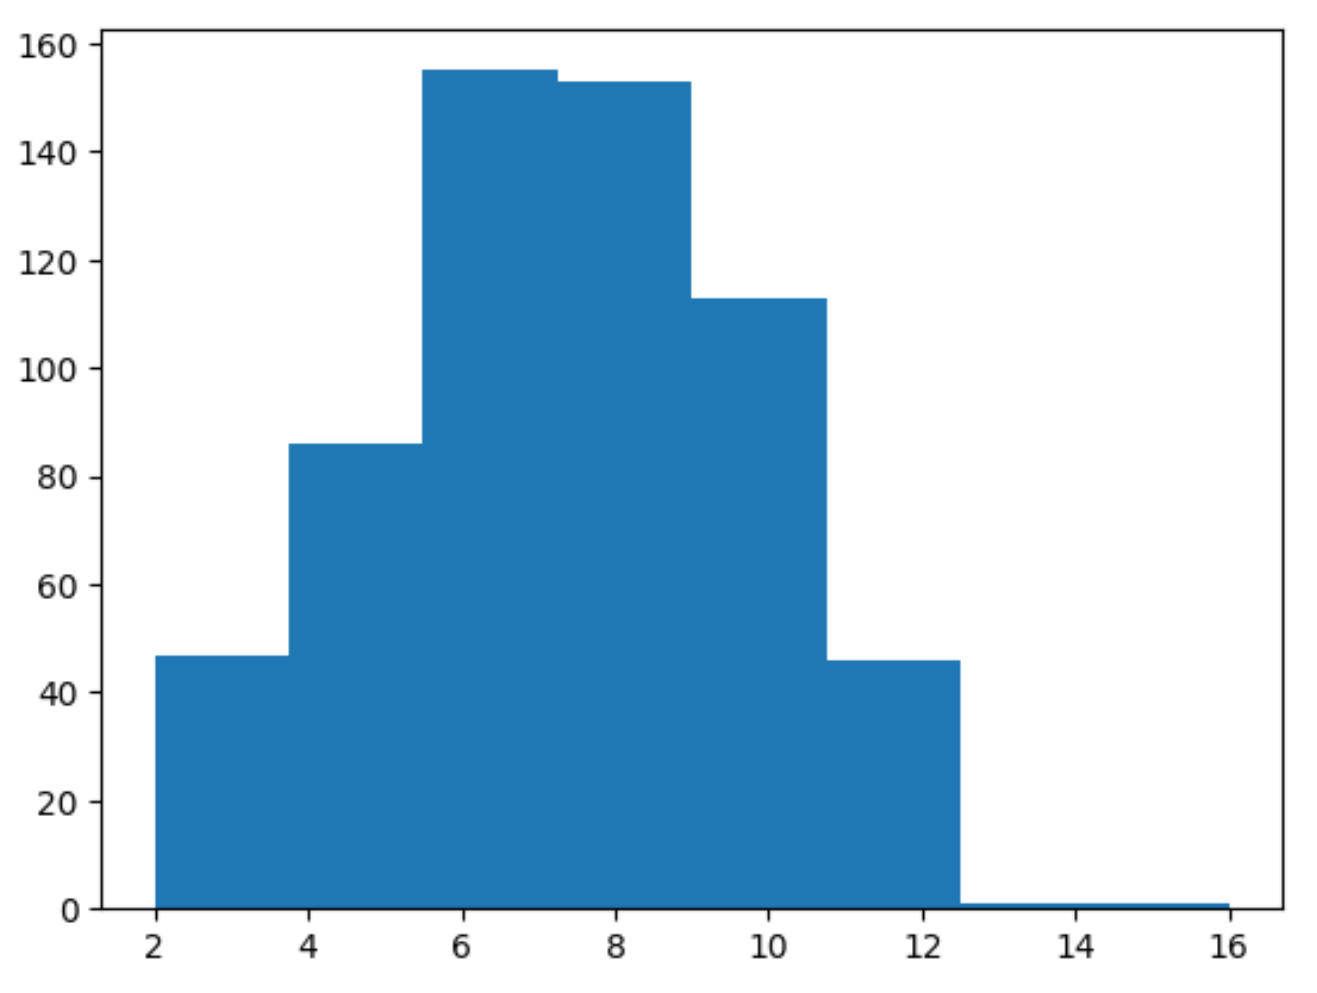
\includegraphics[width=0.9\linewidth]{sections/hist.png}
%     \caption{The statistics of minimal action number for all test cases in \blocksworld}
%     \label{fig:hist}
% \end{figure}


\section{Related work: world model and planning}
\label{sec:related_planning}
Recent years have witnessed successful applications of planning algorithms~\cite{sekar2020planning}, such as AlphaZero~\cite{silver2017mastering}, and MuZero~\cite{schrittwieser2020mastering}. These algorithms are typically based on tree-structured search and are designed to effectively maintain the balance of exploration and exploitation. Knowledge of transition dynamics is the prerequisite for planning, and recent research on model-based reinforcement learning propose to learn a world model (or dynamics model) to plan or assist policy learning. To improve sample efficiency, previous research attempts to learn a world model from offline trajectories, and directly learn a policy within the world model \cite{ha2018recurrent, ha2018world}. With latent imagination in a world model, RL agents can be trained to solve long-horizon tasks~\cite{hafner2019dream, hafner2020mastering}. Besides, the world model is also shown to be helpful to physical robot learning~\cite{wu2023daydreamer}. In this paper, we use LLMs as world models and apply a planning algorithm to search for a reasoning path. This is similar in spirit to model predictive control \cite{camacho2013model}. Compared with previous works, our framework uses general LLMs as the world model and can be adapted to a wide range of open-domain reasoning tasks. \citet{xiang2023language} propose to train LLMs wih a external world model to gain embodied experience, while RAP focuses on the inference stage and is compatible with any training methods.

\section{Adaptive Prompting}
\label{sec:adaptive}
Through our preliminary experiments, we observed that the performance of LLMs is impacted by the discrepancy in difficulty between demonstration cases and the test cases. In the case of RAP, when a new state is predicted, we reformulate the remaining task as a new test case, initialized with the predicted new state. This new test case would require a smaller minimum number of actions, leading to a disparity in the distribution of the demonstration cases and the new cases. To mitigate this issue, we pre-compute the intermediate states of the demonstration cases beforehand. During inference, we truncate the trace from the beginning for each new state in an iteration, which reduces the minimum action number of the demonstration cases as the search tree deepens. This technique significantly enhances the performance of RAP, especially for more intricate problems, which are more susceptible to distribution mismatches.

\section{Reward Choice}
\label{sec:reward_appendix}
\begin{table}[t]
    \centering
    \caption{Ablation study on Blocksworld. $R_1$ is action likelihood reward, $R_2$ is task-specific reward, and $R_3$ is self-evaluation reward.}
    % \vspace{5pt}
    \begin{tabular}{c|c|c|c}
    \toprule
        $R_1$ & $R_2$ & $R_3$ & \thead{Success} \\
        \midrule
        \cmark & \cmark & \xmark & 0.88\\
        \cmark & \cmark & \cmark & 0.91\\
        \cmark & \xmark & \xmark & 0.46\\
        \xmark & \cmark & \xmark & 0.21\\
        \xmark & \xmark & \cmark & 0.14\\
        \xmark & \xmark & \xmark & 0.02\\
    \bottomrule
    \end{tabular}
    \vspace{-5pt}
    \label{tab:bw_ablation}
\end{table}
\begin{table}[t]
  % \hspace{0.5cm}
    \centering
    \caption{Ablation study on GSM8k (first 300 examples). $R_1$ is state transition confidence reward, $R_2$ is action likelihood reward, and $R_3$ is self-evaluation reward.}
    \vspace{5pt}
    \begin{tabular}{c|c|c|c|c|c}
    \toprule
        $R_1$ & $R_2$ & $R_3$ & RAP$^{(1)}$ & RAP$^{(10)}$ & +aggr\\
        \midrule
        \cmark & \xmark & \cmark & 0.410 & 0.450 & 0.503\\
        \cmark & \xmark & \xmark & 0.350 & 0.447 & 0.490 \\
        \cmark & \cmark & \xmark & 0.373 & 0.423 & 0.443\\
         \bottomrule
    \end{tabular}
    \vspace{-5pt}
    \label{tab:gsm8k_ablation}
\end{table}
\noindent \textbf{Results.} We conduct comprehensive experiments on rewards for plan generation (Table~\ref{tab:bw_ablation}) and math reasoning (Table~\ref{tab:gsm8k_ablation}). Note that, in both tables, the first row indicates the setting we use in the main experiments. As shown in Table~\ref{tab:bw_ablation}, the combination of action likelihood and task-specific reward (row 1) can significantly outperform the single reward baselines (row 3, 4, 5). Interestingly, adding the self-evaluation reward can further improve the performance slightly (row 2). Furthermore, as the results on the first 300 samples of GSM8k shown in Table~\ref{tab:gsm8k_ablation}, we can see adding either action likelihood (row 3) or self-evaluation (row 1) on top of confidence reward (row 2) can boost the RAP performance of only using confidence reward (row 1) with one iteration, but action likelihood reward downgrades the accuracy with more iterations. The self-evaluation reward leads to the best performance overall. This indicates the importance of self-evaluation reward in guiding reasoning as an effective and computationally efficient prior to exploration.

\noindent\textbf{Self-evaluation and action likelihood.}
The rewards of self-evaluation and action likelihood are of particular interest, as they can be applied to a wide range of reasoning tasks. Generally, the best usage and combination with other rewards require empirical design and understanding of the task nature, and their effectiveness can vary significantly across different tasks. Here, we provide some intuitions behind the reward choices:

(a) For the problems in which one reasoning step is short and structured, the action likelihood can be very indicative. Otherwise, it may be disturbed by unimportant tokens and become unreliable. For instance, a single step within the Blocksworld domain typically adheres to specific patterns (e.g., \textsc{pick/put/stack} a block…), rendering the action likelihood indicative. However, in the math domain, a reasoning step is expressed in natural language sentences, allowing for greater freedom and potentially introducing noise.

(b) For the problems where it’s easier to recognize some errors afterward than avoid them during generation, self-evaluation emerges as a helpful mechanism for enhancing reasoning accuracy. In mathematical reasoning, LLMs may struggle to generate a correct reasoning step in the first place, but the detection of calculation or logic errors is more feasible. In Blocksworlds, however, assessing the quality of a candidate action is not straightforward and still requires multi-step reasoning. This characteristic diminishes the accuracy of the self-evaluation reward, making it less helpful especially given that likelihood already provides a good intuition for search.
